\newpage
\section{Cálculos sobre infraestructuras}
\label{anexo:infraestructuras}

Los cálculos de la construcción de la infraestructura dependen de muchos factores, entre ellos la fecha de la obra o el tiempo máximo que pueda durar, así como sus dimensiones son factores que llegan a afectar mucho al precio de la misma. Por ello se considerará que ante la ausencia de un plano del local se realizará una estimación aproximada del coste de la obra, por ello se tomará como referencia un precio medio que se puede encontrar en las páginas web de las empresas FIXr \cite{fixr} y Zaask \cite{zaask} puesto que coincide con lo que se ha encontrado durante la investigación y se puede considerar una buena aproximación a lo que sería el precio final de la obra.

\subsection{Cálculo del precio de los accesorios específicos}

\textbf{\textit{Puesto que estos cálculos son necesarios para los siguientes, se realizarán primero.}}

Debido a motivos de seguridad se considera necesario la instalación de ciertos mecanismos de seguridad definidos a continuación.

\subsubsection{Bicicletas Eléctricas}
En el caso de las bicicletas eléctricas se considera que es necesario instalar algún tipo de estructura donde poder encadenarlas y así evitar posibles robos. Se ha escogido el modelo \textbf{Soporte 5 bicicletas} de la marca \textbf{Btwin} (Decatlon) \cite{decathlons5b}, porque se considera que es el que mejor se adapta a nuestras necesidades manteniendo una buena relación calidad/precio, con un coste de 54,99 \glssymbol{euro} por unidad.

También se debe contar con el precio del candado, se ha escogido como mejor opción el \textbf{Candado para bicicletas en U 920 Elops} de la marca \textbf{Elops} \cite{decathloncb}, por su facilidad de uso, por contar con un soporte para la bicicleta (que asegura que no pueda molestar al repartidor) y por su buena relación calidad/precio, que supone un coste de 29,99 \glssymbol{euro} por unidad.

\subsubsection{Patinetes Eléctricos}
En el caso de los patinetes eléctricos se considera necesario instalar una estructura para poder encadenarlos, al igual que con las bicicletas, en este caso la opción que se ha considerado óptima se trata del \textbf{Aparcapatinetes Manuales} de la marca \textbf{Adosa} \cite{aparcapatinetes} (por desgracia el mercado de los patinetes eléctricos es relativamente reciente y por ello el precio en comparación con los soportes para bicicletas es mucho mas elevado) de un precio de 288,61 \glssymbol{euro} para un soporte de  \textbf{8 patinetes}.

También se debe contar con el candado, en este caso se ha escogido el candado \textbf{Masterlock candado-esposas patinete negro} de la marca \textbf{Master Lock} pues se considera es el que mejor se adapta a las necesidades con una buena relación calidad/precio, con un coste de 28,99 \glssymbol{euro} por unidad.


\subsection{Cálculo del área necesaria para cada vehículo}

En todos los casos se considera que el acceso desde la calle hasta el aparcamiento ocupará un total de 4 \glssymbol{metrocuadrado} como máximo, así como un espacio de maniobra de 1,5 \glssymbol{metro} en el caso de las motocicletas, y de 1 \glssymbol{metro} en el caso de patinetes eléctricos y bicicletas eléctricas.

\subsubsection{Motocicletas}
Para el calculo del espacio necesario para las motocicletas, y teniendo en cuenta que en las ordenanzas municipales de la ciudad de Málaga \cite{ordmalaga} no se especifica un tamaño mínimo o necesario para el estacionamiento de ciclomotores, se definirá el tamaño de este en relación a cada vehículo que se vaya a aparcar, añadiendo 15 \glssymbol{centimetro} hacia cada lateral del vehículo, para permitir un mínimo de movilidad entre los vehículos, más la distancia de maniobra anteriormente mencionada.

\paragraph{Askoll eS1:}
\label{askolles1}

Medidas: 1830 x 726 x 1036 \glssymbol{milimetro}. \cite{manualmotoe}

Considerando los 15 \glssymbol{centimetro} hacia cada lateral, más 1,5 \glssymbol{metro} de espacio de maniobra, se puede considerar un área total por vehículo de 3330 x 1026 \glssymbol{milimetro}.

\paragraph{KYMCO Agility Carry 50 E5}
\label{agilitycarry50}

Medidas: 1950 x 1145 x 685 \glssymbol{milimetro}. \cite{eliotmotor}

Considerando los 15 \glssymbol{centimetro} hacia cada lateral, más 1,5 \glssymbol{metro} de espacio de maniobra, se puede considerar un área total por vehículo de 3430 x 1445 \glssymbol{milimetro}.

\paragraph{KYMCO AGility Carry 125}
\label{agilitycarry125}

Medidas: 1925 x 695 x 1100 \glssymbol{milimetro}. \cite{motofichas}

Considerando los 15 \glssymbol{centimetro} hacia cada lateral, más 1,5 \glssymbol{metro} de espacio de maniobra, se puede considerar un área total por vehículo de 3425 x 995 \glssymbol{milimetro}.

\subsubsection{Bicicletas Eléctricas}
\label{bicicletaselectricas}

El cálculo del espacio necesario para las bicicletas eléctricas se debe basar en el espacio que ocupará el soporte de estas (definido más abajo), más el tamaño de la propia bicicleta, más el espacio de maniobra.

En el caso del soporte el modelo escogido se cuenta con unas dimensiones de \cite{aparcapatinetes} 1357 x 375 x 250 \glssymbol{milimetro}

En el caso de la bicicleta eléctrica escogida se cuenta con unas medidas de \cite{emoonmedidas}  188 x 117 x 21 \glssymbol{centimetro}

Teniendo en cuenta que se instalará un soporte para bicicletas las medidas a tener en cuenta son 1357 \glssymbol{milimetro} de ancho, 188 \glssymbol{centimetro} de la bicicleta (se considera el soporte despreciable en esta dirección) más 1 \glssymbol{metro} reservado para maniobras de largo, por cada soporte para bicicletas, lo que deja un área por soporte de 1357 x 2880 \glssymbol{milimetrocuadrado}.


\subsubsection{Patinetes Eléctricos}
\label{patineteselectrico}

Al igual que en el caso de las bicicletas, para los patinetes eléctricos se debe tener en cuenta, para el cálculo del espacio, el soporte de estos, el tamaño del propio patinete, más el espacio de maniobra.

En el caso del soporte escogido se cuenta con unas medidas de \cite{aparcapatinetes} 1500 x 900 \glssymbol{milimetro}.

En el caso del patinete eléctrico escogido se cuenta con unas medidas de \cite{cetallerdelpatinetedos} 108 x 43 x 114 \glssymbol{centimetro}.

Teniendo en cuenta que se instalará un soporte para patientes, las medidas a tener en cuenta son 1500 \glssymbol{milimetro} de ancho, 114 \glssymbol{centimetro} de largo del patinete (se considera el soporte despreciable en esta dirección) más el metro reservado para maniobras, lo que deja un área por soporte de 1500 x 2140 \glssymbol{milimetro}.

\subsection{Cálculo del precio de la obra por metro cuadrado}
Se realiza el cálculo del área total ocupada para cada conjunto del vehículo:

\begin{table}[H]
\centering
\begin{tabular}{|l|c|c|c|c|c|}
\hline
Vehículo                  & Área Vehículo/Soporte & NºM* & NºV** & Area Vehículos & Area Total                 \\\hline
Askoll eS1                & 3330 x 1026 \glssymbol{milimetro}        & NA   & 9     & 3330 x 9234 \glssymbol{milimetro} & 30.75 \glssymbol{metrocuadrado} \\\hline
KYMCO Agility Carry 50 E5 & 3430 x 1445 \glssymbol{milimetro}        & NA   & 5     & 3443 x 7225 \glssymbol{milimetro} & 24.87 \glssymbol{metrocuadrado} \\\hline
KYMCO Agility Carry 125   & 3425 x 995 \glssymbol{milimetro}         & NA   & 5     & 3425 x 4975 \glssymbol{milimetro} & 17.04 \glssymbol{metrocuadrado} \\\hline
F.Lli Schiano E-Moon      & 1357 x 2880 \glssymbol{milimetro}        & 5    & 10    & 2714 x 2880 \glssymbol{milimetro} & 7.82 \glssymbol{metrocuadrado}  \\\hline
Infinitron CITYJam Pro    & 1500 x 2140 \glssymbol{milimetro}        & 8    & 20    & 4500 x 2140 \glssymbol{milimetro} & 9.63 \glssymbol{metrocuadrado} \\\hline
\end{tabular}
\caption{Espacio ocupado total por vehículo para la suposición de viajes de 5 \glssymbol{km}.}
\end{table}

\begin{table}[H]
\centering
\begin{tabular}{|l|c|c|c|c|c|}
\hline
Vehículo                  & Área Vehículo/Soporte & NºM* & NºV** & Área Vehículos & Área Total                 \\\hline
Askoll eS1                & 3330 x 1026 \glssymbol{milimetro}        & NA   & 7     & 3330 x 7182 \glssymbol{milimetro} & 23.92 \glssymbol{metrocuadrado} \\\hline
KYMCO Agility Carry 50 E5 & 3430 x 1445 \glssymbol{milimetro}        & NA   & 5     & 3443 x 7225 \glssymbol{milimetro} & 24.87 \glssymbol{metrocuadrado} \\\hline
KYMCO Agility Carry 125   & 3425 x 995 \glssymbol{milimetro}        & NA   & 5     & 3425 x 4975 \glssymbol{milimetro} & 17.04 \glssymbol{metrocuadrado} \\\hline
F.Lli Schiano E-Moon      & 1357 x 2880 \glssymbol{milimetro}        & 5    & 10    & 2714 x 2880 \glssymbol{milimetro} & 7.82 \glssymbol{metrocuadrado}  \\\hline
Infinitron CITYJam Pro    & 1500 x 2140 \glssymbol{milimetro}        & 8    & 16    & 3000 x 2140 \glssymbol{milimetro} & 6.42 \glssymbol{metrocuadrado} \\\hline
\end{tabular}
\caption{Espacio ocupado total por vehículo para la suposición de viajes de 7.5 \glssymbol{km}.}
\end{table}


\textit{*Nº M: Numero máximo de vehículos por soporte.}
\textit{**Nº V: Numero Vehículos.}

Para la opción híbrida se han  considerado siete patinetes y dos motocicletas eléctricas por lo que será necesario: un solo soporte de patienetes (1500 x 2140 \glssymbol{milimetro}) más el espacio para las dos motocicletas (3330 x 2052 \glssymbol{milimetro}), dando un area total de 10.04 \glssymbol{metrocuadrado}.

\subsubsection{Cálculo del precio de la cimentación y el asfaltado del parking}
Se entiende que el precio más representativo para la cimentación es el presentado en Zaask \cite{zaaskpc} donde la media por \glssymbol{metrocuadrado} se establece en torno a los 100 \glssymbol{europormetrocuadrado}. En el caso del asfaltado se utilizará la información recabada de CronoShare \cite{cronoshare} donde se puede obtener un precio medio por \glssymbol{metrocuadrado} de 16 \glssymbol{europormetrocuadrado}. De esta forma se puede calcular un coste total para cimentación y asfaltado de 116 \glssymbol{europormetrocuadrado}. Se debe recordar que hay que añadir los cuatro \glssymbol{metrocuadrado} del acceso a la vía pública.

\begin{table}[H]
\centering
\begin{tabular}{|l|c|c|c|}
\hline
Vehículo                  & Área Párking               & Área Total                 & Precio Total \\\hline
Askoll eS1                & 30.75 \glssymbol{metrocuadrado} & 34.75 \glssymbol{metrocuadrado} & 4031 \glssymbol{euro}       \\\hline
KYMCO Agility Carry 50 E5 & 24.87 \glssymbol{metrocuadrado} & 28.87 \glssymbol{metrocuadrado} & 3348.92 \glssymbol{euro}    \\\hline
KYMCO Agility Carry 125   & 17.04 \glssymbol{metrocuadrado} & 21.04 \glssymbol{metrocuadrado} & 2440.64 \glssymbol{euro}    \\\hline
F.Lli Schiano E-Moon      & 7.82 \glssymbol{metrocuadrado}  & 11.82 \glssymbol{metrocuadrado} & 1371.12 \glssymbol{euro}    \\\hline
Infinitron CITYJam Pro    & 9.53 \glssymbol{metrocuadrado}  & 13.53 \glssymbol{metrocuadrado} & 1572.96 \glssymbol{euro}   \\\hline
\end{tabular}
\caption{Coste de la cimentación y el asfaltado por vehículo para la suposición de viajes de 5 \glssymbol{km}.}
\end{table}

\begin{table}[H]
\centering
\begin{tabular}{|l|c|c|c|}

\hline
Vehículo                  & Área Parking               & Área Total                 & Precio Total \\
\hline
Askoll eS1                & 23,92 \glssymbol{metrocuadrado} & 27,92 \glssymbol{metrocuadrado} & 3.238,72 \glssymbol{euro}    \\
\hline
KYMCO Agility Carry 50 E5 & 24,87 \glssymbol{metrocuadrado} & 28,87 \glssymbol{metrocuadrado} & 3.348,92 \glssymbol{euro}    \\
\hline
KYMCO Agility Carry 125   & 17,04 \glssymbol{metrocuadrado} & 21,04 \glssymbol{metrocuadrado} & 2.440,64 \glssymbol{euro}    \\
\hline
F.Lli Schiano E-Moon      & 7,82 \glssymbol{metrocuadrado}\glssymbol{metrocuadrado}  & 11.82 \glssymbol{metrocuadrado} & 1.371,12 \glssymbol{euro}    \\
\hline
Infinitron CITYJam Pro    & 6,42 \glssymbol{metrocuadrado}  & 10,42 \glssymbol{metrocuadrado} & 1.208,72 \glssymbol{euro}   \\
\hline
\end{tabular}
\caption{Coste de la cimentación y el asfaltado por vehículo para la suposición de viajes de 7,5 \glssymbol{km}.}
\end{table}

En el caso de la opción híbrida, se cuenta con un área de parking de 10,04 \glssymbol{metrocuadrado}, más los 4 \glssymbol{metrocuadrado} del acceso a la vía pública, lo que nos da un total de 14,04 \glssymbol{metrocuadrado}, por un total de 1628,64 \glssymbol{euro}.

\subsubsection{Cálculo del precio de la instalación de una pérgola para la protección contra sol y lluvia}

\begin{figure}[ht]
    \centering
    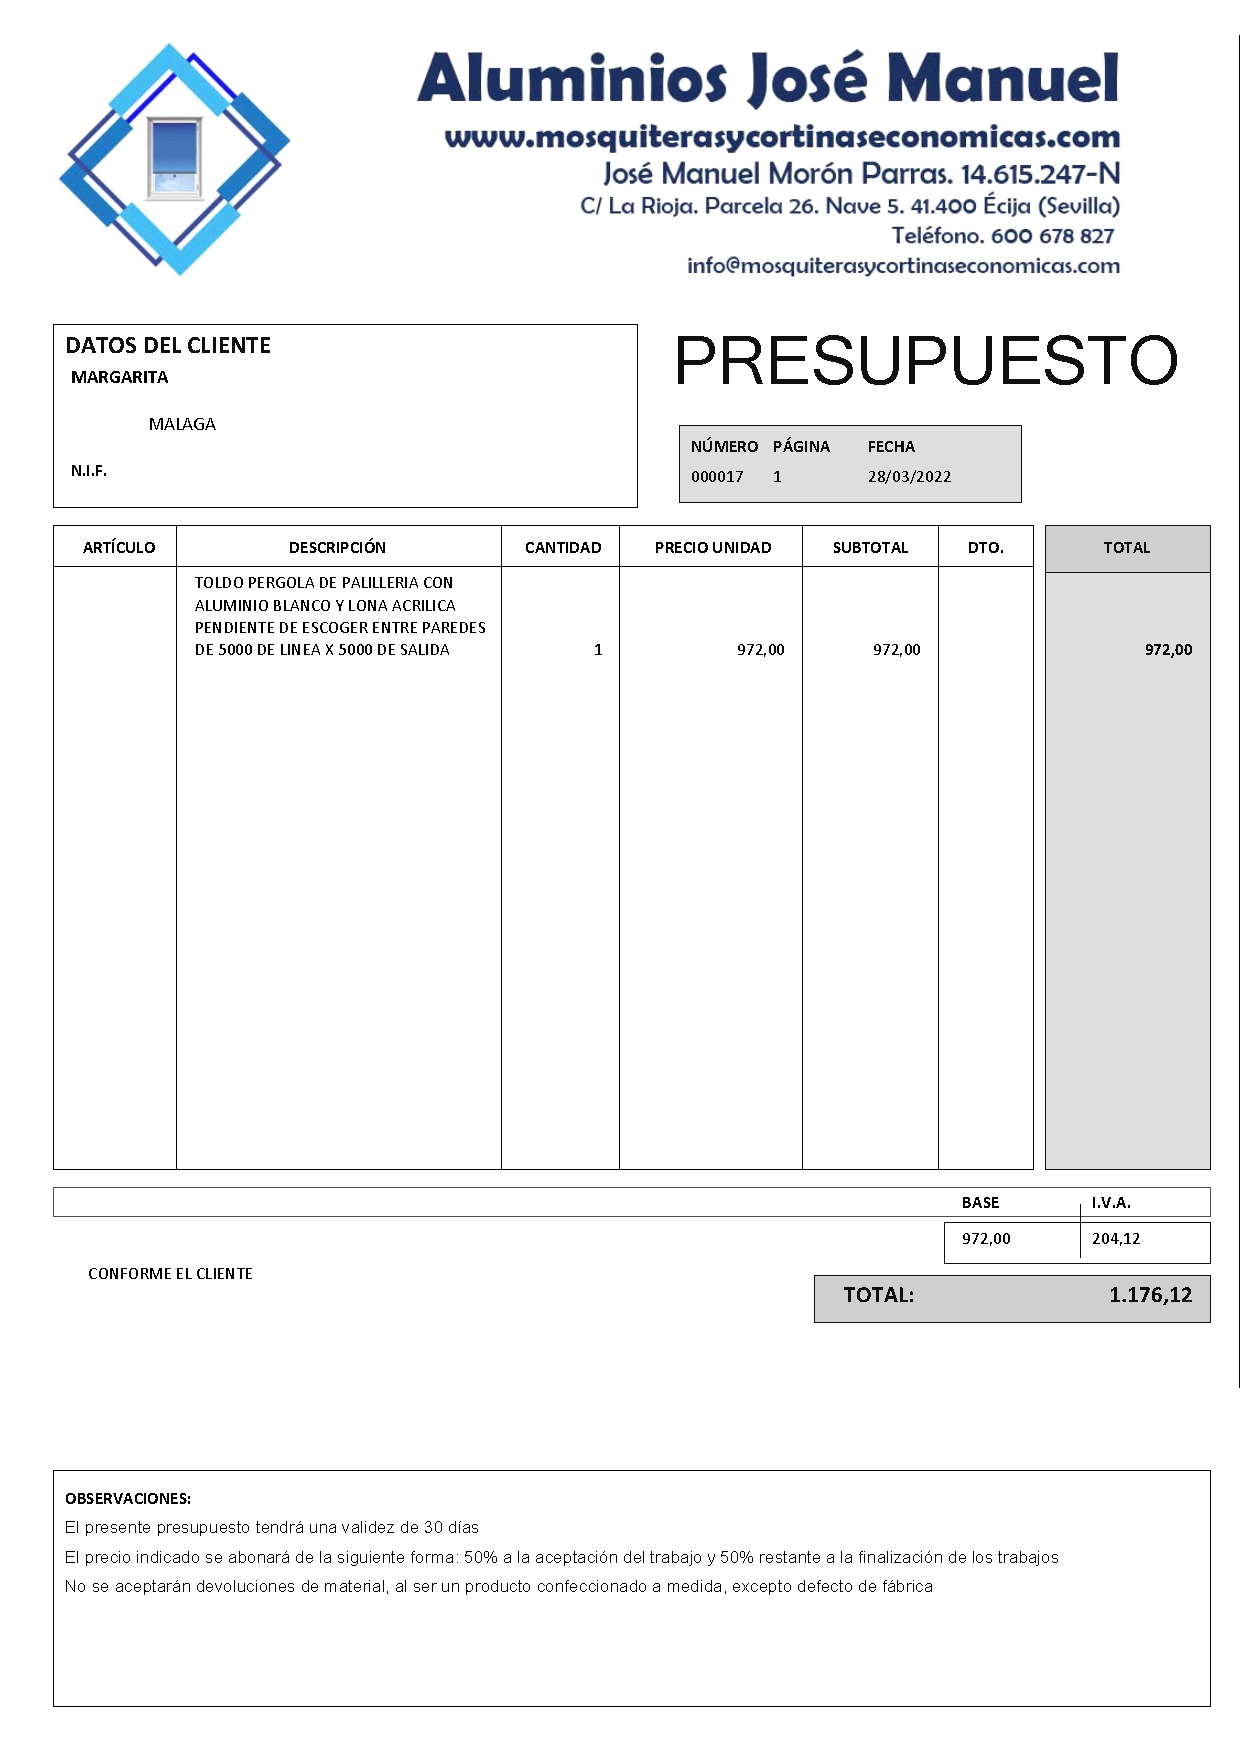
\includegraphics[scale = 0.45]{contenido/Anexos/Presupuesto 1-000017.pdf}
    \caption{Presupuesto pérgola aluminio.}
    \label{fig:PresupPA}
\end{figure}

Considerando el presupuesto que se ha obtenido y que se puede observar en la \autoref{fig:PresupPA} se puede estimar el precio medio de una pérgola como: 1176,12 \glssymbol{euro} / 25 \glssymbol{metrocuadrado} = 47,05 \glssymbol{europormetrocuadrado}. Dando un total para cada modelo de:

\begin{table}[H]
\centering
\begin{tabular}{|l|c|c|}
\hline
Vehículo                  & Área Pérgola               & Precio Total \\\hline
Askoll eS1                & 30,75 \glssymbol{metrocuadrado} & 1.446,79 \glssymbol{euro}    \\\hline
KYMCO Agility Carry 50 E5 & 24,87 \glssymbol{metrocuadrado} & 1.170,13 \glssymbol{euro}    \\\hline
KYMCO Agility Carry 125   & 17,04 \glssymbol{metrocuadrado} & 801 \glssymbol{euro}       \\\hline
F.Lli Schiano E-Moon      & 7,82 \glssymbol{metrocuadrado}  & 367,93 \glssymbol{euro}     \\\hline
Infinitron CITYJam Pro    & 9,53 \glssymbol{metrocuadrado}  & 448,39 \glssymbol{euro}    \\\hline
\end{tabular}
\caption{Precio de instalación de Pérgola para vehículos con supuesto de 5 \glssymbol{km}.}
\end{table}

\begin{table}[H]
\centering
\begin{tabular}{|l|c|c|}
\hline
Vehículo                  & Área Pérgola               & Precio Total \\\hline
Askoll eS1                & 23,92 \glssymbol{metrocuadrado} & 1.125,43 \glssymbol{euro}    \\\hline
KYMCO Agility Carry 50 E5 & 24,87 \glssymbol{metrocuadrado} & 1.170,13 \glssymbol{euro}    \\\hline
KYMCO Agility Carry 125   & 17,04 \glssymbol{metrocuadrado} & 801 \glssymbol{euro}       \\\hline
F.Lli Schiano E-Moon      & 7,82 \glssymbol{metrocuadrado}  & 367,93 \glssymbol{euro}     \\\hline
Infinitron CITYJam Pro    & 6,42 \glssymbol{metrocuadrado}  & 302,06 \glssymbol{euro}    \\\hline
\end{tabular}
\caption{Precio de instalación de Pérgola para vehículos con supuesto de 7,5 \glssymbol{km}.}
\end{table}

Para el modelo híbrido, se cuenta con con un área de parking de 10,04 \glssymbol{metrocuadrado} que equivale a un total de 489,32 \glssymbol{euro}.

\subsubsection{Cálculo del precio de la instalación de un garaje cerrado (prefabricado)}
Considerando los precios estudiados en Fixr \cite{fixrgaraje} (2000 \glssymbol{euro} para una garaje cerrado de 15 \glssymbol{europormetrocuadrado}) se puede estimar un precio medio de 133,33 \glssymbol{europormetrocuadrado}. Dando un total por modelo de:

\begin{table}[H]
\centering
\begin{tabular}{|l|c|c|}
\hline
Vehículo                  & Area Garaje                & Precio Total \\\hline
Askoll eS1                & 30,75 \glssymbol{metrocuadrado} & 4.099,90 \glssymbol{euro}    \\\hline
KYMCO Agility Carry 50 E5 & 24,87 \glssymbol{metrocuadrado} & 3.315,92 \glssymbol{euro}    \\\hline
KYMCO Agility Carry 125   & 17,04 \glssymbol{metrocuadrado} & 2.271,94 \glssymbol{euro}    \\\hline
F.Lli Schiano E-Moon      & 7,82 \glssymbol{metrocuadrado}  & 1.042,64 \glssymbol{euro}    \\\hline
Infinitron CITYJam Pro    & 9,53 \glssymbol{metrocuadrado}  & 1.270,63 \glssymbol{euro}   \\\hline
\end{tabular}
\caption{Precio de instalación de Garaje para vehículos con supuesto de 5 \glssymbol{km}.}
\end{table}

\begin{table}[H]
\centering
\begin{tabular}{|l|c|c|}
\hline
Vehículo                  & Área Garaje                & Precio Total \\\hline
Askoll eS1                & 23,92 \glssymbol{metrocuadrado} & 3.189,25 \glssymbol{euro}   \\\hline
KYMCO Agility Carry 50 E5 & 24,87 \glssymbol{metrocuadrado} & 3.315,92 \glssymbol{euro}    \\\hline
KYMCO Agility Carry 125   & 17,04 \glssymbol{metrocuadrado} & 2.271,94 \glssymbol{euro}    \\\hline
F.Lli Schiano E-Moon      & 7,82 \glssymbol{metrocuadrado}  & 1.042,64 \glssymbol{euro}    \\\hline
Infinitron CITYJam Pro    & 6,42 \glssymbol{metrocuadrado}  & 855,98 \glssymbol{euro}    \\\hline
\end{tabular}
\caption{Precio de instalación de Garaje para vehículos con supuesto de 7,5 \glssymbol{km}.}
\end{table}

Para el modelo híbrido, se cuenta con un área de parking de 10,04 \glssymbol{metrocuadrado} que equivale a un total de 1.338,63 \glssymbol{euro}.

\subsection{Cálculo del precio de la instalación eléctrica}
En caso de contar con vehículos eléctricos se debe contar con puntos de carga para estos, en este caso se debe tener en cuenta que todos los vehículos presentados cuentan con un cargador para baterías que se puede conectar directamente a una toma de corriente.

\subsubsection{Intalación eléctrica para exteriores (caso pergola)} El coste de una instalación eléctrica para exteriores, según se estima en Zaask \cite{zaaskiem} se encuentra entre 700 y 1.550 \glssymbol{euro}, puesto que necesitaríamos varias tomas y les daremos mucho uso, asumiremos el precio máximo para asegurarnos la máxima calidad posible, 1.550 \glssymbol{euro}.

\subsubsection{Instalación eléctrica para interiores (caso garaje)} Considerando que la instalación eléctrica de interior requiere menos medidas de seguridad, consideraremos que el precio de esta será siempre inferior a la instalación exterior por lo que tomaremos el punto medio de 1.000 \glssymbol{euro}.

\newpage
% \addcontentsline{toc}{section}{Referencias}
% \section*{Referencias}
% \label{referencias_nucleo}
% \makeatletter
% \def\@bibitem#1{\item\if@filesw \immediate\write\@auxout
%   {\string\bibcite{#1}{A\the\value{\@listctr}}}\fi\ignorespaces}
% \def\@biblabel#1{[A{#1}]}
% \makeatother
% \printbibheading[title={Referencias},heading=bibintoc]
\nocite{*}
\newrefcontext[labelprefix=\thesection.]
\printbibheading[title={Referencias},heading=subbibintoc]
\printbibliography[heading=none,resetnumbers=true,keyword=infraestructura]
\label{applastpage}
